\section{Work Done}
  In this next section I will discuss the work that was carried on the project. In our team we have \textit{'ways of working'}
  flowchart that helps guides us in how the project should be done throughout the team (GoRetro, 2023). Our ways of working is broken down into 5 sections, 
  all of which will be discussed.

  \begin{figure}[H]
    \centering
    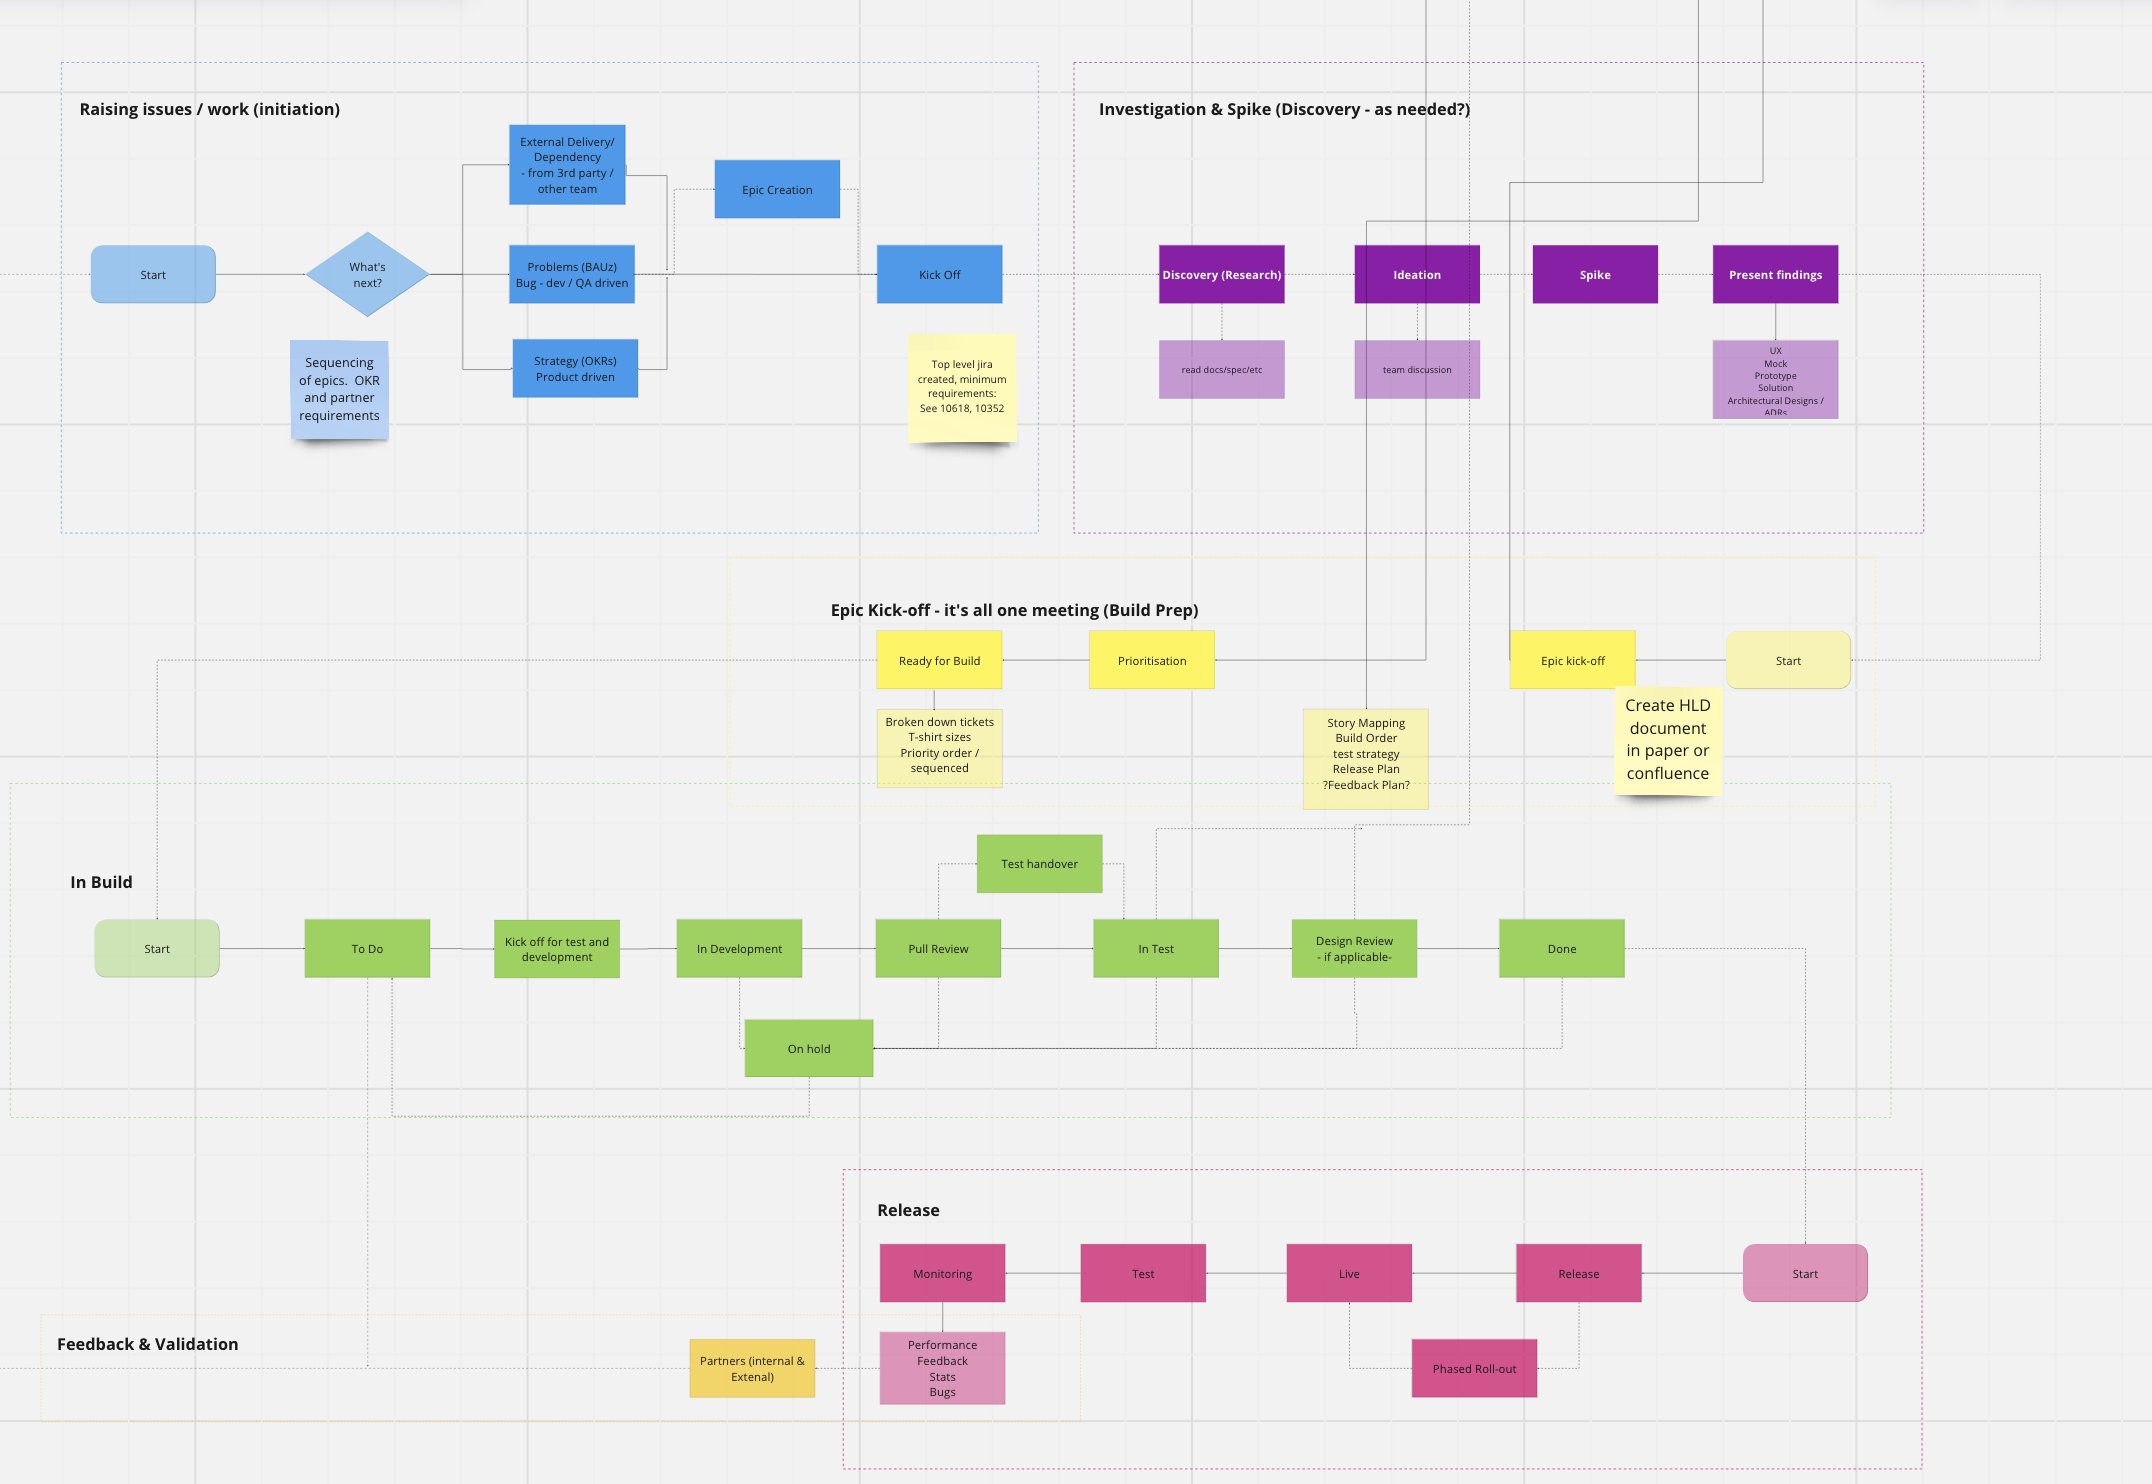
\includegraphics[width=12cm]{assets/workflow/fullWorkflow.png}
    \caption{Full ways of working flow diagram used by SpaceChimp.}
    \label{fig:fullWorkflow}
  \end{figure}

  \footnote{\textbf{B1} - This section shows how a systematic approach to software development was used for the project.}
  \footnote{\textbf{SE-S01} - This section will discuss the build, architecture and changes to initial design, task creation and release strategies.}
  \footnote{\textbf{SE-S06} - Through this section it will be demonstrated how we assure quality by sticking to our ways of working. This includes testing, 
  code reviews, releasing and monitoring software.}
  \footnote{\textbf{SE-K03} - This section and the diagram in the appendix shows our ways of working which was followed during the project.}
  \footnote{\textbf{SE-K05} - This section also steps through how the system was designed, developed and deployed to AWS.}

  \newpage

  \subsection{Requirements and epic creation}
  The First stage is initiation, what's the project going to be about, how it fits into the companies strategy and OKRs, requirement gathering 
  and epic creation, an epic being a set of user stories/features (Karolis, Saulius, 2023).

  \begin{figure}[H]
    \centering
    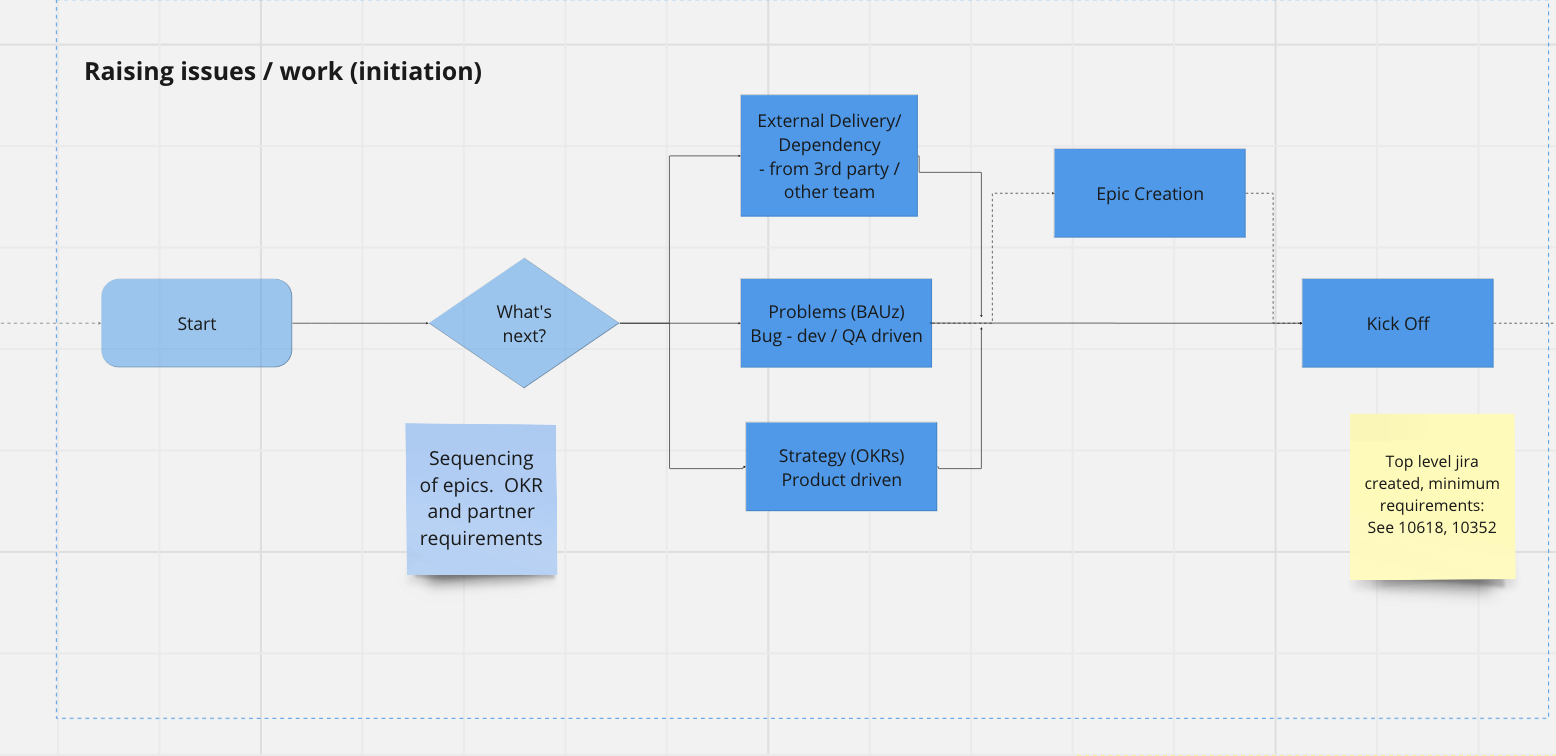
\includegraphics[width=8cm]{assets/workflow/initiate.png}
    \caption{Initiation stage of our ways of working.}
    \label{fig:workflowInitiate}
  \end{figure}

  Due to complications in project allocation, I was not involved in the initial phases of development for this project. However discussions with 
  people that were, highlighted that due to the lack of external partner interaction their wasn't much to discuss and no solid requirements were 
  outlined, only the goal which is to allow the schedule generator to be moved from a static refresh of schedules to an event driven process.

  The benefits of the project and how it achieves our OKRs has been discussed previously in the report. However I want to create some tangible
  requirements here using the MoSCoW framework which consists of must, should, could and won't haves (Eduardo, 2022). I will focus on software requirements and 
  denote whether they are functional (F) or non-functional (NF) (Bigelow 2020).

  \begin{enumerate}
    \item (F) The software \textbf{Must} be able to process schedule updates. 
    \item (F) The software \textbf{Must} be able to process episode updates.
    \item (F) The software \textbf{Must} be able to process ancestor updates.
    \item (NF) The software \textbf{Must} keep stored data more relevant than the static version.
    \item (F) The software \textbf{Must} still support a coldstart option.
    \item (F) The software \textbf{Must} contain alarms to alert us to errors.
    \item (F) The software \textbf{Should} gather metrics on processing time and types of updates.
    \item (F) The software \textbf{Should} clean up unneeded data from it's store.
    \item (NF) The software \textbf{Could} support parallelised processing.
  \end{enumerate}

  \footnote{\textbf{SE-K02} - Although there wasn't any solid requirements captured by the team, I have broken down the project into it's requirements
  to demonstrate what this could have looked like.}
  \footnote{\textbf{P5} - There were no external partners discussions for this project due to it being a change to an internal system. However the
  following text simply describes this process and conflict management.}
  
  In this case requirement gathering was easy as there were no partners to discuss the changes with as it's all internal and the output to partners
  stays the same. If this wasn't the case then requirements would have to be gathered from all partners affected or interested in the projects 
  outcome. These requirements would be gathered through meetings and conversations with these partners individually and compromises may have to 
  be made by both sides.
  This is usually the case when there is a requirement conflict, which can be described as:
  \begin{quote}
    \textit{'Requirements conflict is defined as unexpected or contradictory interaction between requirements that has a negative 
    effect on the results (Cameron, Velthuijsen, cited in Kim et al, 2007)'}
  \end{quote}
  These conflicts need to be managed well, as Kim et al (2007) warns these conflicts can \textit{'lead 
  to negative or undesired operation of the system'}. However certain stakeholders will often carry more leverage than another, taking into 
  consideration the Pareto Principle (Sanders, 1987), the 80-20 rule, it's easy for an organisation to leave out requirements of smaller stakeholders.
  A balance must be struck here where all parties are kept happy, without damaging the original idea of the project when large stakeholders try 
  and morph it into what they deem it should be.

  In this case no conflicts occurred due to the how internalised the project is. An epic was created in Jira and these requirements could then be explored 
  and implemented in the next phase.

\newpage
  \subsection{Investigation and spike}
  After initiation the project is investigated and then \textit{spiked}. In this case investigation/research for the most part has been done,
  as we knew the system was feasible due to following the same design as our catalogue pipeline. However it was determined that a spike of the 
  proposed algorithm would be done.

  \begin{figure}[H]
    \centering
    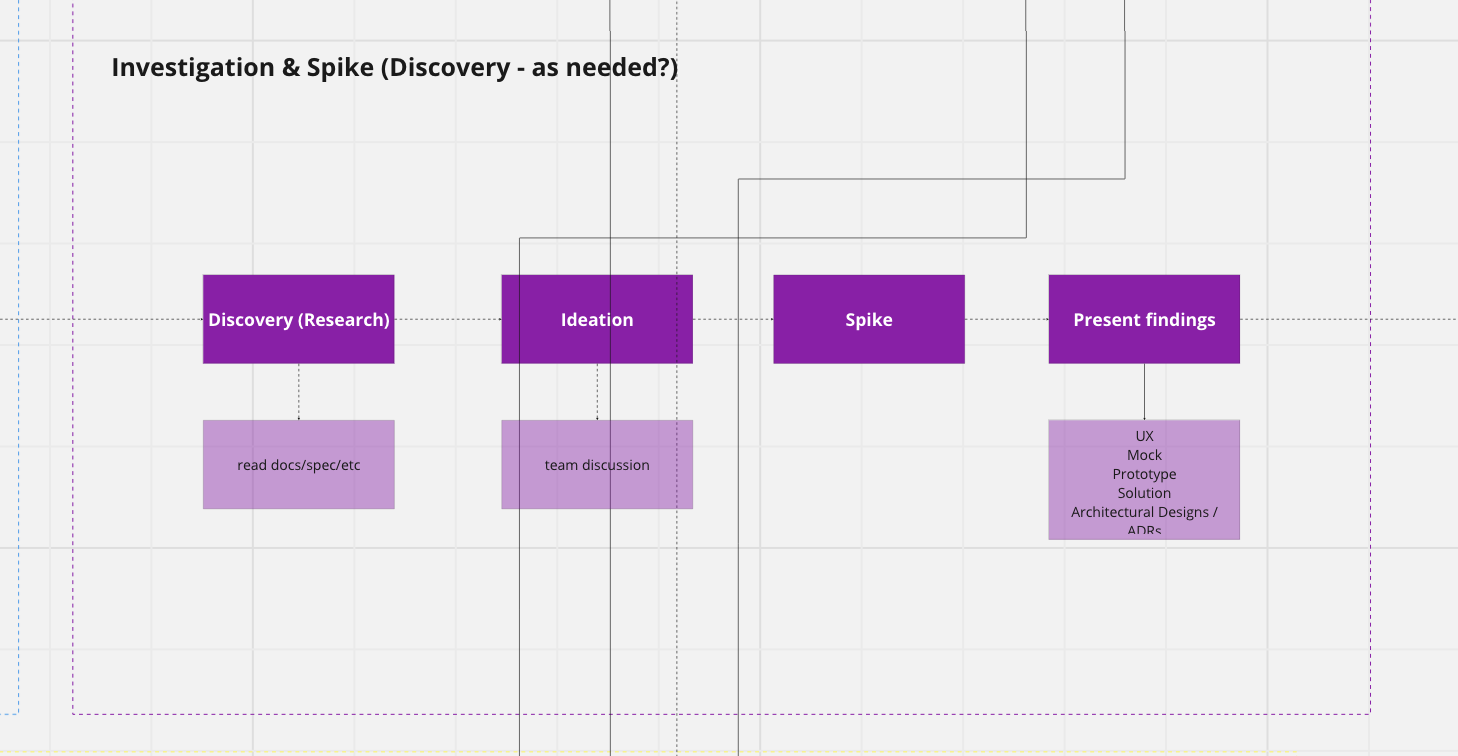
\includegraphics[width=8cm]{assets/workflow/investigation.png}
    \caption{Investigation stage of our ways of working.}
    \label{fig:workflowInvestigation}
  \end{figure}

  A spike is often used when there are unknowns about a  project (Visual Paradigm, 2024). A study done by 
  Hashimi and Gravell (2020) found that a majority of people in industry saw spikes as an effective tool and helped in managing risks. In another
  study they also stated that one of key purposes of a spike was to help guide story/ticket estimations (Hashimi, Gravell, 2019). 

  In the first paper it was also hypothesised that technical debt can also be lowered through the use of spikes, with technical debt be defined as:
  \begin{quote}
    \textit{'the idea that developers sometimes accept
    compromises in a system in one dimension (e.g., modularity) to meet an
    urgent demand in some other dimension (e.g., a deadline)' (Kruchten et al, 2012)}
  \end{quote}

  Spikes were used by Glas and Hedén (2021) to help bring down technical debt in their study. However when thought about simply, 
  a spike could be seen as a tool to spot the technical debt before it touches live systems. Due to a prototype being made flaws can be spotted 
  early and ironed out before the \textit{'real'} development work begins.

  For the project a spike was carried out to test the algorithms outlined in \hyperref[sec:AppendixC]{\textbf{Appendix C}} to test the 
  throughput of the system and see if it could handle the incoming requests. We used the technical spike template recommended by Microsoft (2021), to 
  document findings and outline the spikes objectives. Hashimi, Abduldaem and Gravell (2022) found that  \textit{'timeboxing, objectives,
  documentation, and clear communication'} were the key factors that lead to a successful spike.

  There was no time limit set, which did lead to scope creep (Martins, 2023) and more time being spent than was necessary. It's important to remember that a 
  spike is not meant to be the final product, however scope creep lead to the spike being almost a fully working system, albeit unrefined and with issues. 
  This is something as a team we have now changed in our process and will always time-box spikes in the future to prevent this.

  Despite this the other key factors were well adhered to. Objectives and documentation of the spike were put into a spike document
  and we had communication with a more senior member of the team at all times as well as daily stand ups to communicate issues/progress on the spike. 
  \footnote{\textbf{P4} - This section demonstrates self-direction and originality to improve a design created by a more senior developer.}
  \footnote{\textbf{SE-S02} - This section also demonstrates the evaluation of the design and recommends both current and future improvements that can be made.
  In this case cloud technologies such as lambda and dynamoDB are recommended in the spikes output.}
  The full spike document can be seen in \hyperref[sec:AppendixD]{\textbf{Appendix D}}, below are the key findings.

  \begin{enumerate}
    \item A garbage collector should be used to clean up data that is no longer referenced by a schedule. This will help lower the amount of redis sets/gets
    and has no negative affect on partners.
    \item When a catalogue item (episode/series/brand) updates it will also need to update it's associated schedules, for titling and descriptions. This in 
    itself is not a problem, however if the number of schedules referenced is large it can significantly slow the system down. Parallelisation should be 
    looked into, at least at the schedule level to help ease this. Full parallelisation would require a new design to support parallelised editing of the 
    broadcast list held in episodes (this discussed in the \hyperref[sec:storageSolutions]{\textbf{Research}} section).
    \item Redis duplication is complex and is only needed so that episodes can reference a list of schedules that they are in. Might be worth using 
    DynamoDB here as this will also help with parallelisation (This is explored in the \hyperref[sec:future]{\textbf{Future Work}} section).
    \item Additional filtering from the catalogue pipeline could be added to only send updates for items that are referenced by a schedule. This would 
    stop lambda being ran that essentially do nothing, this is also discussed in \hyperref[sec:future]{\textbf{Future Work}}.
  \end{enumerate}

  \footnote{\textbf{P5}- Discussion were had during and after the spike presentation to come to the following decisions.}
  It was determined by the team that, for now, the system should be single-threaded and stick to the original design due to time constraints.
  Parallelisation could be looked into in the future when we had some time. However it was agreed for a garbage collector to be used and 
  when a batch of schedule updates is is triggered by a catalogue update that some form of concurrency would be required. This can be done with schedule
  objects due to the single threaded nature of the current system. As the schedule updates are being done because of a catalogue update the only 
  fields that can change are the titles and descriptions. These do not affect or reference anything other than the object itself.

  \begin{figure}[H]
    \centering
    \includegraphics[width=8cm]{diagrams/activity/Schedule Concurrency.png}
    \caption{Simple activity diagram showing basic concurrency logic for updating schedules triggered by a catalogue update.}
    \label{fig:scheduleConcurrency}
  \end{figure}

\newpage
  \subsection{Slicing and kick-off}
  Another small section is the \textit{'kick-off'}, usually a single meeting where the team gets together and discusses the tickets that makeup
  the project as a whole. 

  \begin{figure}[H]
    \centering
    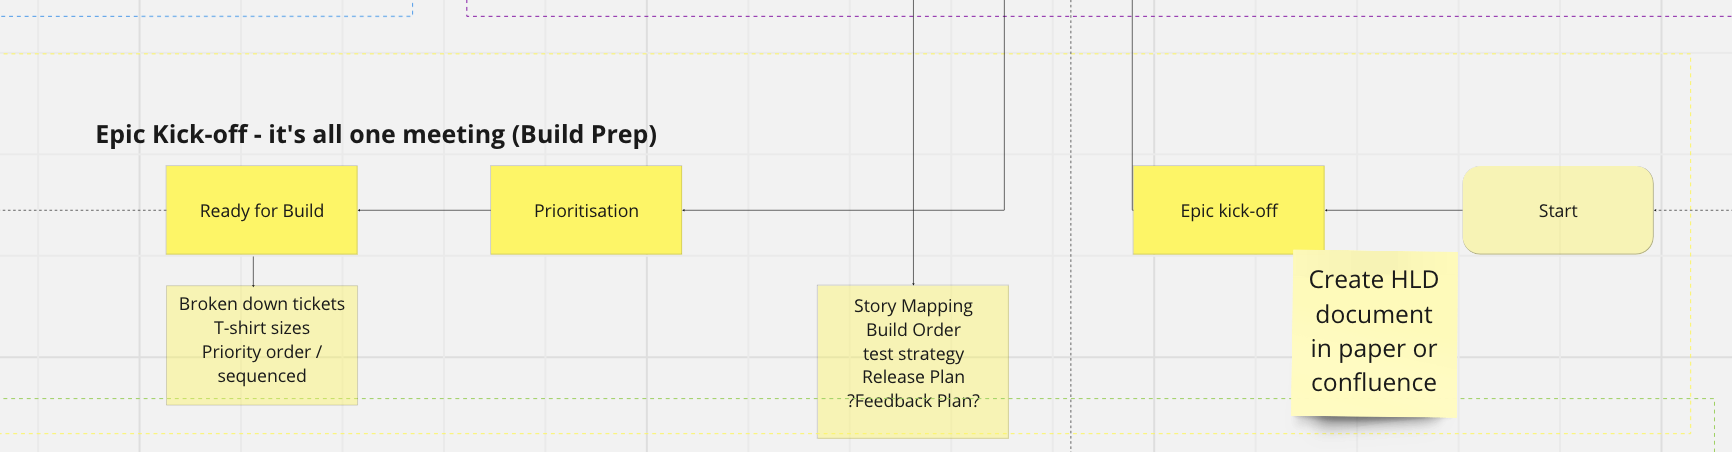
\includegraphics[width=8cm]{assets/workflow/kickoff.png}
    \caption{Kick-off stage of our ways of working.}
    \label{fig:workflowKickOff}
  \end{figure}

  Ideally this work has already been broken down into tasks. This is where the spike really helps, instead of guessing we are able to better understand 
  the work that needs doing and create tasks accordingly (Hashimi, Abduldaem, Gravell, 2022). The following diagram shows the initial breakdown of 
  tasks/tickets that were created for the project.

  \begin{figure}[H]
    \centering
    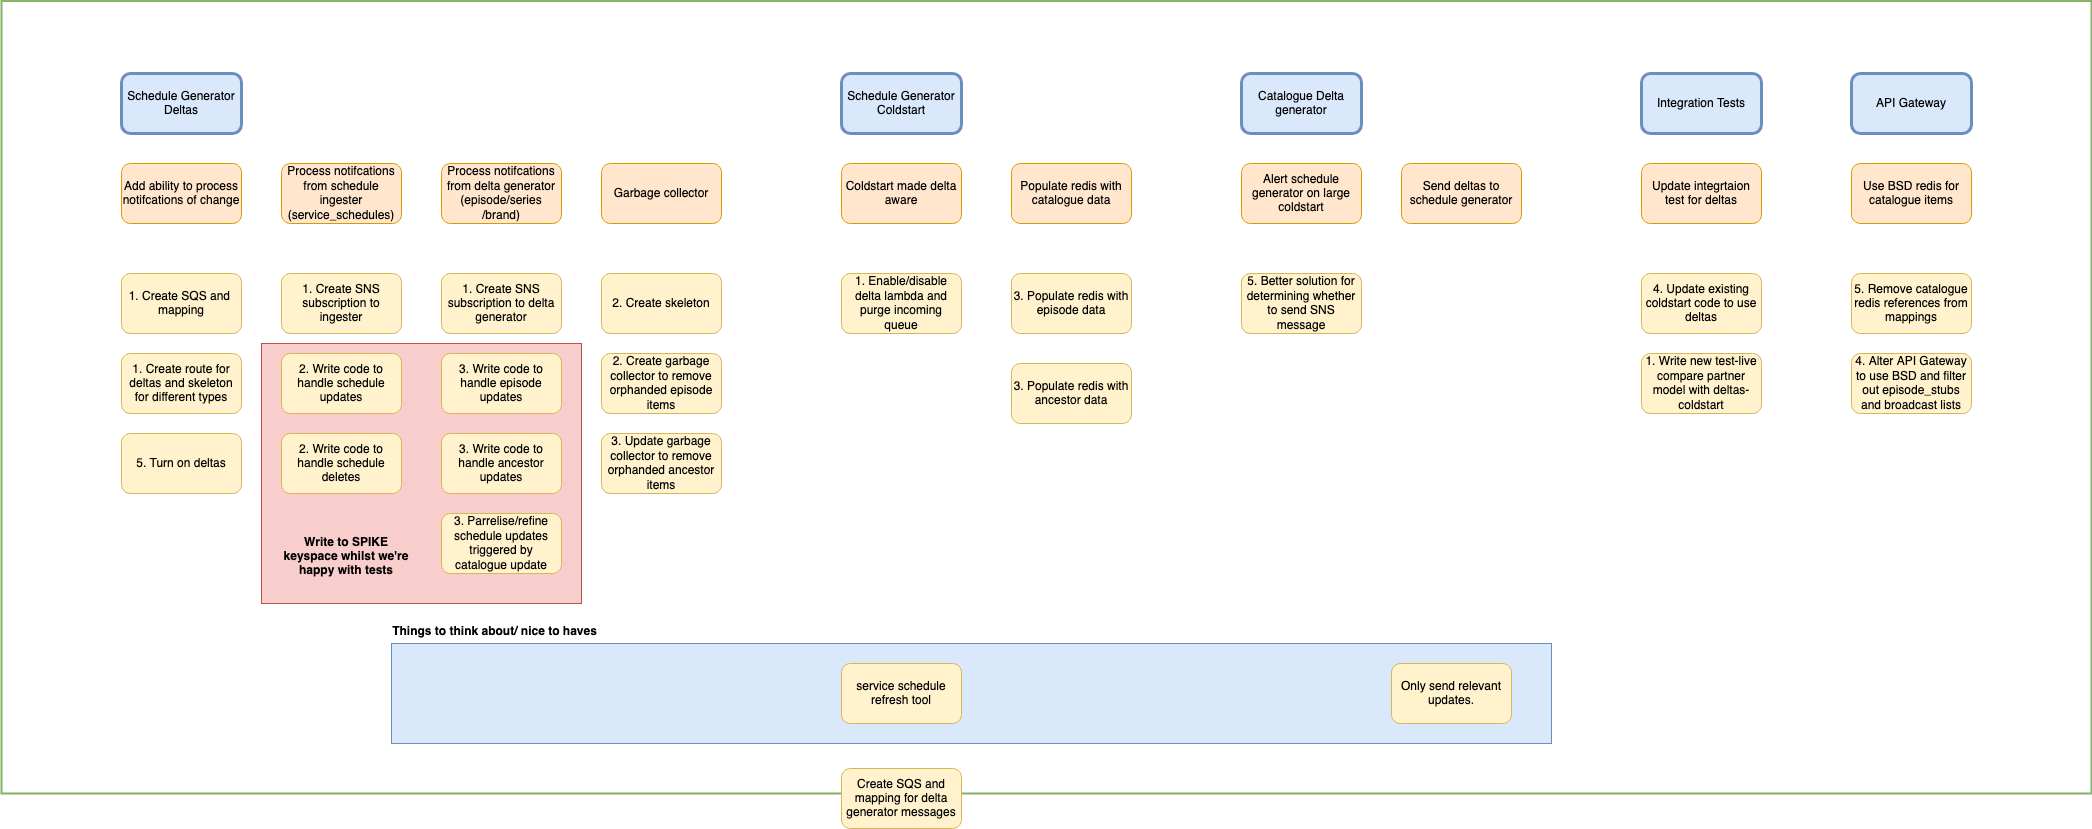
\includegraphics[width=14cm]{assets/schedulesSlicing.drawio.png}
    \caption{Pre-work slicing of work, organised vertically into components.}
    \label{fig:schedulesSlicing}
  \end{figure}

  A work breakdown structure (WBS) is a tool used to \textit{'break down deliverables into sub-deliverables to visualize projects'} (Raeburn, 2024) 
  and is typically broken down into 3 levels, parents, dependencies and sub-tasks, however it can consist of as any as a team wants. For the above I kept it 
  at 3 levels, going vertically, blue represents self-contained features/components, orange is a parent task to complete the feature and yellow is a 
  sub-task of the parent task. Numbers on the sub-tasks represent the initial prioritisation/ordering of the tasks into slices or feature sets.

  It's important to note that this is not the final list of tasks. Unknowns will always appear whilst developing the software and result in additional
  tasks being created. However the WBS helps refine the scope to what is needed (Burghate, 2018). As can be seen in the above figure there are 3 tasks that have 
  been moved to a \textit{'nice to have'} section, which have been deemed unnecessary for the projects initial completion.

  Another way to visualise these feature sets is using an Archimate implementation and migration diagram. This allows the modelling of work packages,
  gaps, deliverables, plateaus (stages) and events (The open group, 2016). The diagram on the next page shows the project mapped out using these elements, 
  documenting the deliverables for each feature set.

  \begin{figure}[H]
    \centering
    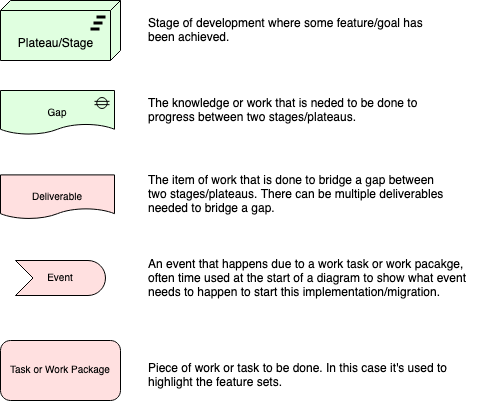
\includegraphics[width=6cm]{assets/migrationKey.drawio.png}
    \caption{Implementation and migration diagram components (The open group, 2016 and Jonkers et al, 2011).}
    \label{fig:migrationKey}
  \end{figure}

  \newpage

  \begin{landscape}
    \begin{figure}
      \centering
      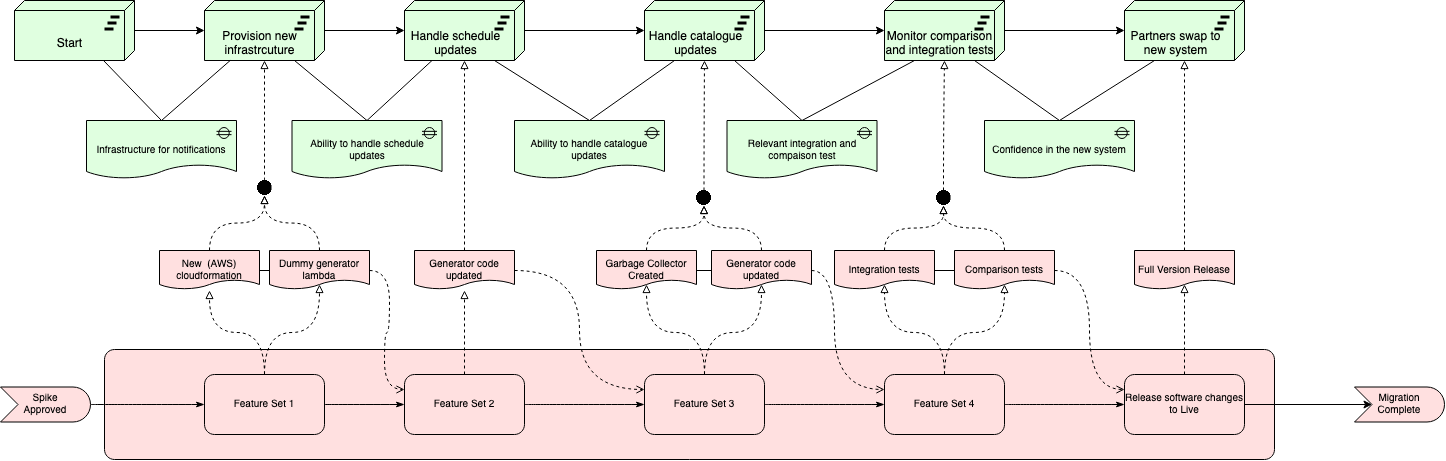
\includegraphics[width=20cm]{assets/migration.drawio.png}
      \caption{Figure showing Archimate implementation/migration diagram for project.}
      \label{fig:migration}
    \end{figure}
  \end{landscape}

\newpage
  \subsection{Build software}
  Before discussing the build stage, it's important to understand the multiple environments used in development.

  \begin{figure}[H]
    \centering
    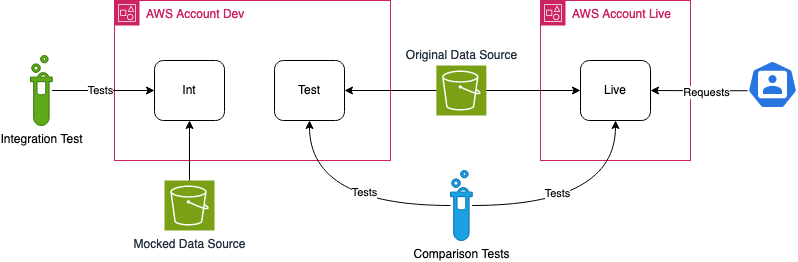
\includegraphics[width=8cm]{assets/environments.drawio.png}
    \caption{Diagram showing the different environments used by SpaceChimp.}
    \label{fig:environments}
  \end{figure}

  The above figure illustrates where the pipelines get their data from dependant on the environment, as well as what tests access said environment.
  We have 3 environments, int, test and live, with test mimicking live (Wiggins, 2017). This allows us to use the test environment to protect live from 
  any bugs or errors introduced by a task whilst also allowing the testing of outputs between old and software (Zheng, 2021). However, when running on test
  and live we don't have control over the data source and the events it sends out to the pipeline, thus making it hard to test certain scenarios and features.
  This is where the int environment is used, we mock the data source used on test/live but have full control over what is added and removed. This allows 
  us to routinely check all edge cases and features are working as expected.

  \vspace{0.2cm}

  The build stage consists of writing and testing the software and resembles the flow of our Kanban board.

  \begin{figure}[H]
    \centering
    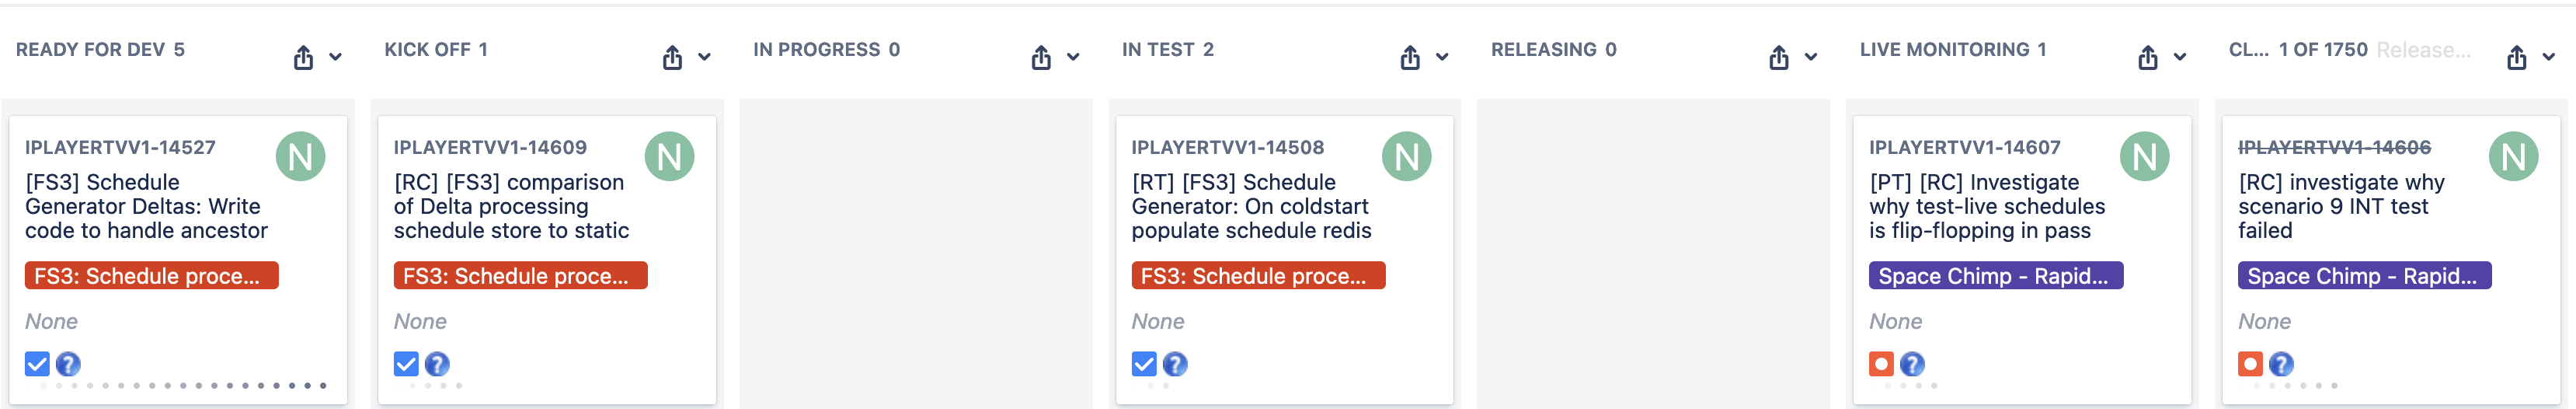
\includegraphics[width=10cm]{assets/kanbanBoard.png}
    \caption{SpaceChimps Kanban board, descriptions can be seen in \hyperref[sec:AppendixE]{\textbf{Appendix E}}.}
    \label{fig:kanbanBoard2}
  \end{figure}

  \begin{figure}[H]
    \centering
    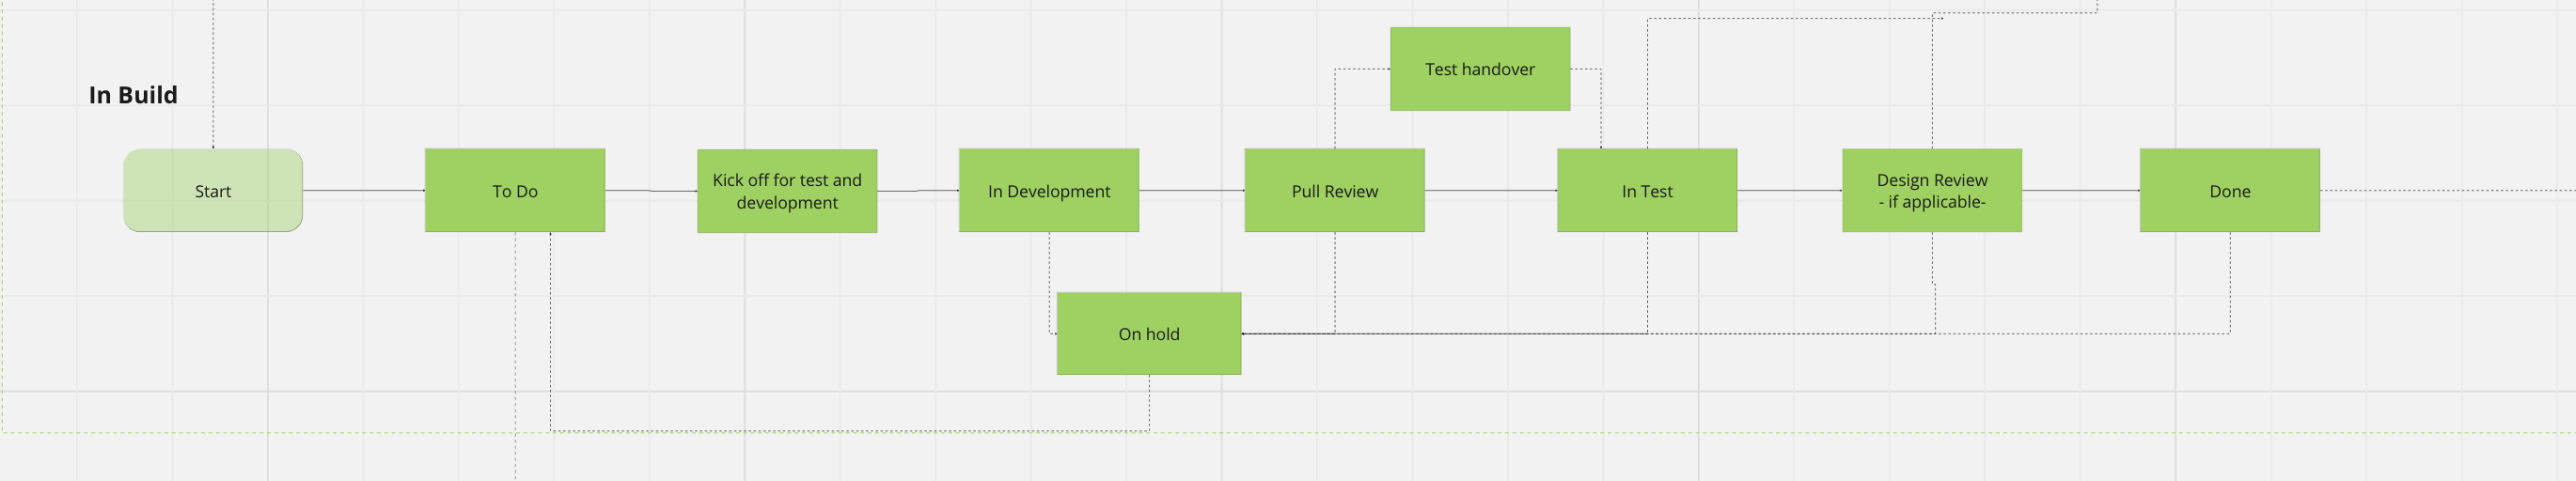
\includegraphics[width=8cm]{assets/workflow/build.png}
    \caption{Build stage of our of ways of working.}
    \label{fig:workflowBuild}
  \end{figure}

  I will now discuss the 4 key components/features that were built during this stage, along with decisions and challenges that occurred during development.

  \newpage
  \subsubsection{Delta/change lambda}
  Before notification events were being processed, schedules relied on the coldstarting/refreshing of data every 15 minutes. The delta lambda is 
  the component that moves away from this paradigm and is the main component in this project. I have separated this section into the different types
  of notifications the component can receive, schedule updates and deletes and catalogue updates and deletes. But before delving into that, a bit of extra
  information is required about the build.

  \vspace{0.2cm}
  In the old system there was no link between episodes and schedules. We now need one, as certain changes to episodes can change what a schedule 
  contains. For this reason, it was decided that a new field could be added to episode, the broadcast\_list field. This would contain a list of all 
  schedules that an episode was referenced in.

  In addition to this, an architectural decision was made, before me taking on the project for this report, to have all schedule documents be in one keyspace,
  this can be seen in \hyperref[sec:AppendixF]{\textbf{Appendix F}}. 
  This making it easy to return all the relevant data on partner requests from our API and now with an additional field, making it so catalogue schemas would 
  not have to be changed. To do this all data relating to any current schedules offered must be copied over from the catalogue Redis keyspace to the schedule
  Redis keyspace, with the broadcast\_list field being added only to the schedule's version of the object. The below figure shows how this works on a
  schedule update.

  \begin{figure}[H]
    \centering
    \includegraphics[width=12cm]{diagrams/activity/Populate Catalogue Items.png}
    \caption{Activity diagram showing logic of populating schedule Redis.}
    \label{fig:scheduleRedisPopulationActivity}
  \end{figure}

  There are 3 outcomes that can happen here:
  \begin{enumerate}
    \item If the episode is already in the schedules store, then we need to add a link to the current schedule being updated if it doesn't
    already reference it. 
    \item If it's not in the schedules store, but is in the catalogue store, then it needs to be copied over and have the current schedule
    being updated referenced in its broadcast list.
    \item If it's not in either store, then a stub must be made, this stub has a unique identifier (pid), a type of \emph{episode\_stub} and 
    a broadcast list, that in this case holds the schedule currently being updated.
  \end{enumerate}

  The episode stub is required, despite it containing no useful information to the schedules tilting and other fields and is also discarded when a
  partner requests a schedule. It is required because of the event driven nature of the new system and the broadcast list it contains. With a stub in 
  the store, when an episode update is processed for that stub, it can now also update all the schedules associated with it, immediately populating tilting
  and descriptions.

  As will be discussed in the following sections, different types of notifications can affect different kinds of data. Below is a table showing the 
  relations between types of updates and what can be affected. The garbage collector will be discussed later in the report but is also included in 
  the table for completeness.

  \begin{table}[H]
    \centering
    \begin{tabular}{|p{0.3\textwidth}|p{0.15\textwidth}|p{0.15\textwidth}|p{0.15\textwidth}|}
      \hline
      & Schedule & Episode & Ancestor \\ \hline
      Schedule Update & \ding{51} & \ding{51} \ding{55} & \ding{51} \\ \hline
      Schedule Delete & \ding{55} & \ding{55} & \\ \hline
      Episode Update & \ding{51} & \ding{51} & \ding{51} \\ \hline
      Ancestor Update & \ding{51} &  & \ding{51} \\ \hline
      Garbage Collector &  &  & \ding{55} \\ \hline
    \end{tabular}
    \caption{Table showing how different types of notification can affect stored data (\ding{51} updates, \ding{55} deletes).}
  \end{table}


  \newpage
  \paragraph{Schedule Updates}
  \footnote{\textbf{SE-K04} - The following section shows countless diagrams showing how the internal system functions.}
  Schedule updates refer to either the updating of a schedule, or the creation of a new schedule. There are some guards around whether the 
  schedule exists, then all catalogue data associated with the schedule is copied from the catalogue store to the schedule store, if it's 
  not already there. This data can then be used to transform everything into the final schedule, where if any valid changes have been made, the 
  new schedule is stored.

  \begin{figure}[H]
    \centering
    \includegraphics[width=8cm]{diagrams/activity/Schedule Update.png}
    \caption{Activity diagram showing logic when schedule update notification received.}
    \label{fig:scheduleUpdateActivity}
  \end{figure}

  There is an edge case specified in the above diagram, where a broadcast within a schedule changes the episode that it's going to play. 
  In this case we must either tidy up the old episodes broadcast list to no longer contain a reference to the schedule, or, if that episode no 
  longer references any schedules, remove it from the schedule store.

  \begin{figure}[H]
    \centering
    \includegraphics[width=8cm]{diagrams/activity/Broadcast Changed.png}
    \caption{Activity diagram showing logic to handle broadcast episode change.}
    \label{fig:broadCastChangeActivity}
  \end{figure}

  \newpage
  \paragraph{Schedule Deletes}
  Schedule deletes are one of the simpler events. Other than some basic guards to check objects exists in Redis, all episode object referenced in 
  the schedule's broadcasts have the schedule being deleted removed from their broadcast list. If this list is empty, then that episode is also removed
  from the schedule store. After all this is done, the schedule is also removed from the schedule store.

  \begin{figure}[H]
    \centering
    \includegraphics[width=8cm]{diagrams/activity/Schedule Delete.png}
    \caption{Activity diagram showing logic when schedule delete notification received.}
    \label{fig:scheduleDeleteActivity}
  \end{figure}

  \newpage
  \paragraph{Catalogue Updates}
  Catalogue updates must also be processed by the schedule generator as they contain information about titling, programme descriptions and more.

  \begin{figure}[H]
    \centering
    \includegraphics[width=6cm]{diagrams/activity/Episode Update.png}
    \includegraphics[width=6cm]{diagrams/activity/Ancestor Update.png}
    \caption{Activity diagrams showing logic when episode (left) and ancestor update (right) notifications received.}
    \label{fig:scheduleUpdateCatalogueActivity}
  \end{figure}

  Episode and ancestor updates are similar. Episode updates must update themselves but also that episode's parents as
  the parents contain additional tilting information required for the schedule to be accurate.

  Due to this titling information being held at multiple levels of the catalogue data, when an ancestor is updated it must update itself
  and then find all episodes in the schedule store that are dependent on it.

  Episodes contain a list of schedules that reference it. These schedules must be updated, so a method was created that could handle these
  schedule changes in a batch form.

  \begin{figure}[H]
    \centering
    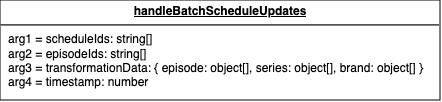
\includegraphics[width=8cm]{assets/handleBatchScheduleInterface.drawio.png}
    \caption{Class diagram showing the interface for the handling schedule updates triggered by catalogue notifications.}
    \label{fig:catalogueTriggeredScheduleUpdateClass}
  \end{figure}

  \footnote{\textbf{SE-K04} - Class diagram and parameter breakdown shows how shared modules can be planned in advance to not create 
  blockades in workflow.}

  The method used the above interface and could be called the same way when updating an episode or an ancestor. The data includes:
  \begin{itemize}
    \item \textbf{scheduleIds} - Schedules in episodes broadcast lists.
    \item \textbf{episodeIds} - Episodes effected by the change, singular on episode update, multiple on ancestor update.
    \item \textbf{transformationData} - Episode/series/brand data needed to transform schedules.
    \item \textbf{timestamp} - Used for consistent update time on all updates.
  \end{itemize}

  Using this interface logic can then carried out to only update the broadcasts that have changed within a schedule instead of the 
  entire schedule itself.

  \begin{figure}[H]
    \centering
    \includegraphics[width=6cm]{diagrams/activity/Catalogue update triggered schedule updates.png}
    \caption{Activity diagram showing logic that happens when a catalogue notification triggers schedule updates.}
    \label{fig:catalogueTriggeredScheduleUpdateActivity}
  \end{figure}

  \paragraph{Catalogue Deletes}
  It was determined during the spike that catalogue deletes would not need to be processed due to the creation of the garbage collector removing 
  orphaned ancestor items, and schedule events taking care of episode removals. This saves a lot of additional lambda invokes over time.

  \newpage
  \subsubsection{Coldstarts}
  We use the term coldstart to refer to the refreshing of all data, in schedules terms all schedules will be checked to see if an update has occurred.
  This is not related to a cold start/boot in relation to serverless architectures (Microsoft Azure, 2018), although this is something that can affect 
  our lambdas. We already had a coldstart in place, but changes would have to be made to work with the new delta/notifications environment.

  \begin{figure}[H]
    \centering
    \includegraphics[width=8cm]{diagrams/activity/Intial Coldstart Design.png}
    \caption{Activity diagram showing initial idea for coldstart changes.}
    \label{fig:initialColdstart}
  \end{figure}

  The above diagram shows the initial design for how the coldstart would function. The changes seem relatively simple:
  \begin{enumerate}
    \item Disable triggering of lambda on delta notification event. This is so no changes can interfere with the refresh of data.
    \item Purge the queue of updates before starting processing to stop unnecessary triggers of the lambda after the cold start has finished.
    \item Populate the Redis with all the catalogue data it needs, this is done on schedule updates also. 
    \item Re-enable the triggering of lambda on delta notification event.
  \end{enumerate}

  Disabling and enabling of the lambda trigger can be achieved through the UpdateEventSourceMapping api (Amazon Web Services, 2024j) provided by AWS. 
  At the start, the trigger can be disabled, then re-enabled once the coldstart is finished.

  \begin{figure}[H]
    \centering
    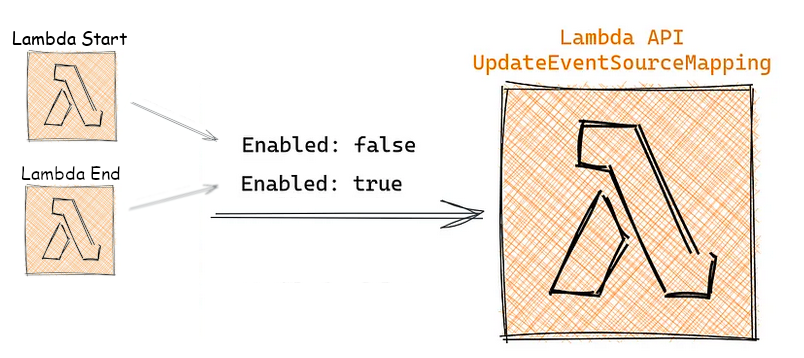
\includegraphics[width=8cm]{assets/lambdaMapping.png}
    \caption{Diagram edited from Charles (2021) to show lambda mapping states.}
    \label{fig:lambdaMapping}
  \end{figure}

  Purging the SQS queue of delta notifications can also be done though a similar API and the population of Redis is already done per schedule, so 
  this seems like an easy switchover to work in the new world of delta notifications.

  However, as work began the code grew more and more complex, due mainly to the new logic of copying data over into the new schedule Redis keyspace.
  Maintaining the broadcast list in the episodes would mean making the population logic complex and hard to follow. Code complexity can be a huge 
  problem with developers not wanting to edit the code in fear of breaking the current workings, difficulty to maintain 
  (Mateus, Andre, 2022 and Olbrich et al, 2009) and the \textit{truck/bus factor} which illustrates how hard it would be for a new team member to 
  understand with no help from the creator (Avelino et al, 2016). In addition to this, a study done by (Taibi et al, 2017) found that 
  \textit{'Smells related to size and complexity are considered harmful by a higher percentage of participants than others.'}. The system created is 
  complex and has multiple inputs that can interfere with each other, the same study also found that this higher complexity is less likely to be 
  refactored in the future (Taibi et al, 2017).

\begin{table}[H]
  \centering
  \begin{tabular}{|l|llr|}
  \hline
  \multicolumn{1}{|c|}{\multirow{2}{*}{Complexity}} & \multicolumn{3}{l|}{Level of occurrence (\%)}                        \\ \cline{2-4} 
  \multicolumn{1}{|c|}{}                            & \multicolumn{1}{l|}{Seldom} & \multicolumn{1}{l|}{Regularly} & Often \\ \hline
  Low                                               & \multicolumn{1}{l|}{7.94}   & \multicolumn{1}{l|}{23.81}     & 57.14 \\ \hline
  Medium                                            & \multicolumn{1}{l|}{12.70}  & \multicolumn{1}{l|}{55.56}     & 19.05 \\ \hline
  High                                              & \multicolumn{1}{l|}{46.03}  & \multicolumn{1}{l|}{28.57}     & 14.29 \\ \hline
  \end{tabular}
  \end{table}

  For these reasons a new approach was thought of. The coldstart would tidy up the differences between its \textit{truth} the internal store, and 
  it's output. Anything not in the internal store is to be removed with the rest of the schedules being processed as if it was a delta notification 
  event.

  \begin{figure}[H]
    \centering
    \includegraphics[width=8cm]{diagrams/sequence/Final Coldstart.png}
    \caption{Sequence diagram showing the new flow of the final coldstart solution.}
    \label{fig:finalColdstart}
  \end{figure}

  This allows the re-use of existing code whilst reducing the complexity and potential code duplication of the coldstart by a sizeable amount.

  \newpage
  \subsubsection{Garbage Collector}
  Nowadays garbage collectors are synonymous with programming languages such as Java (Xu et al, 2019), however the first language to implement garbage 
  collection was LISP in the 1960s (Matam, 2023). Before then programmers had to manually assign memory for variables stored on the heap, as well as 
  unassign the memory when they were finished using it (Fakhoury et al, 2024 and Matam, 2023). 
  Garbage collection stops memory leaks as any unused memory is reclaimed (Microsoft, 2023).

  Whilst doing the spike it was thought that a form of \textit{garbage collector} may help simplify some of the logic around the removal of catalogue items
  from Redis. Episode were easy to remove as once their associated broadcast list was empty, they no longer needed to be stored. But due to having to 
  traverse upwards to find other linked items, it became complex and time consuming to calculate if an episode's parents (series) and grandparents (brands)
  also needed to be removed from the schedule Redis store.

  \begin{figure}[H]
    \centering
    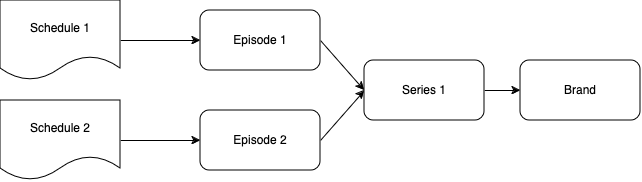
\includegraphics[width=8cm]{assets/catalogueTree.drawio.png}
    \caption{Example tree and associations between objects.}
    \label{fig:catalogueTree}
  \end{figure}

  Looking at the figure above outlines one possible scenario. If \emph{Episode 1} is removed from \emph{Schedule 1} then the episode object should be removed
  from Redis and so should its parent \emph{Series 1} as that also no longer has any schedule relations. However, \emph{Brand} must stay as it still
  has \emph{Episode 2} and \emph{Series 2} that depend on it and relate it to \emph{Schedule 2}. Due to the potential to fan out like this, all data stored
  in the Redis keyspace would have to be checked to see if there was any schedule still depending on the top-level object (the brand). This takes a lot of
  memory and bandwidth to retrieve all this data. It was for that reason that it was decided, once a day a garbage collector should be ran to 
  tidy up anything no longer required.

  \begin{figure}[H]
    \centering
    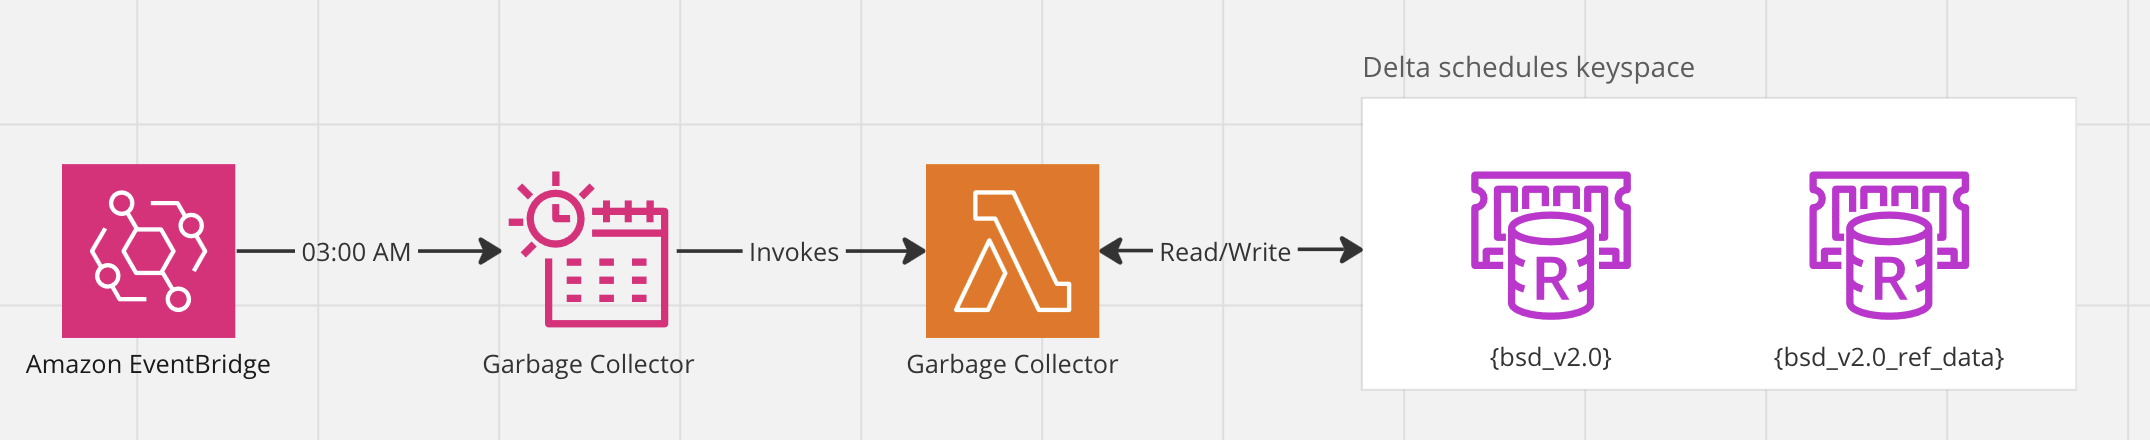
\includegraphics[width=8cm]{assets/architectures/garbageCollector.png}
    \caption{Garbage collector architecture.}
    \label{fig:garbageCollectorArchitecture}
  \end{figure}

  Above is the final architecture, a lambda is triggered by a scheduler once a day a 3AM to tidy up the leftover series and brands. In a later
  \hyperref[sec:garbageCollectorConsolidation]{\textbf{section}} the idea of moving all catalogue removals, including episodes, to the garbage 
  collector is explored.

  \newpage
  \subsubsection{End-to-end tests}
  \footnote{\textbf{SE-S01} - This section discusses test coverage which is vital in enterprise code.}
  In this section I want to discuss the larger tests that were created as part of the project. These include end-to-end (e2e) and comparison tests.
  As a team we follow the pattern of tests laid out in the test pyramid below.

  \begin{figure}[H]
    \centering
    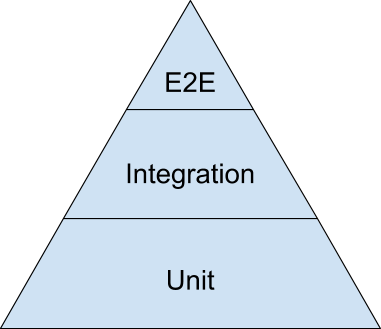
\includegraphics[width=6cm]{assets/testPyramid.png}
    \caption{Test pyramid (Wacker, 2015).}
    \label{fig:testPyramid}
  \end{figure}

  Unit tests and integration tests are written alongside the code and can run on project build as they are cheap and quick to run (Spinellis, 2017).
  E2e tests sit at the top of this pyramid and should be used sparingly. This is not always the case, in other types of development, for example mobile,
  this pyramid can be turned upside down (Knott, 2015, cited in Contan, Dehelean and Miclea, 2018). This is probably due to mobile application being 
  primarily UI driven, which is the opposite for this project.

  In addition to this e2e and integration tests often get confused with one another. Integration tests \textit{'ensure synchronization between modules'}
  (Testim, 2021), and are more comparable to a unit test. Whereas a unit test is concerned on a single function/method an integration would test the calling of 
  methods by other methods and ensure integration between these two functions are working as expected. E2e tests are focused on actions/events that the 
  system must deal with as normal operation and could be described as automated manual testing (Testim, 2021).
  
  Due to their higher complexity, e2e tests are not without their potential problems. These include maintenance the written 
  tests, flakiness (are prone to randomly pass or fail without any discernible reason), time taken to run the tests and the cost of both the 
  execution of the tests and the time to write them (Yang and Leotta et al, 2023). 

  One of the larger problems we've faced in the past is asynchronicity between tests (Leotta et al, 2023). For example, if we upload a schedule at the 
  start of the pipeline and want to test its structure at the end of the pipeline where partners would receive it, there's a lot that can interfere with 
  expected outputs. For the most part these bugs are when tidy up of a previous test is not carried out fully. If two test use the same identifier 
  for a schedule and then don't remove said schedule, this can result in tests not running how expected. It's for this reason during the development 
  of these new tests the code below was written to ensure that the schedule item about to be asserted on is not stored in the Redis prior to the 
  test starting.

  \begin{lstlisting}[caption=Code to ensure schedule to asserted on is not present at the start of the test.]
    waitFor(`Ensure ${schedule} is not present before running test`, async () => {
      const bsd = await fetchFromRedis({
        command: 'isAbsent',
        keySpace: 'bsd_v2.0',
        sidDates: [schedule],
      })
      expect(bsd).toEqual([null])
    })
  \end{lstlisting} 

  Our current tests are written in \textit{scenarios} by our test team.
  Currently these cover all possible scenarios, however, have a lot of overlap and repetitiveness. In an ideal world a test would cover an individual
  use case (Daly, 2022). These 14 scenarios could then be a part of these use case tests which would speed how quickly they run, thus lowering the cost.
  These use cases could be the following:

  \begin{itemize}
    \item Update a schedule
    \item Delete a schedule
    \item Update an episode
    \item Update an ancestor (series/brand)
    \item Tidy up orphaned items in Redis (garbage collector)
  \end{itemize}

  This lowers the number of running test by 9 and removes a lot of time and duplication taken by setting up the scenarios. Due to time constraints and 
  prioritisation of other projects for the future, this refactor has not yet been undertaken but is in the backlog of things to do in the future. The 
  cost saved from changing this wouldn't be high and doesn't justify the time it would take to refactor.

  For this project we stuck with the scenarios, some had already been done in previous work which meant we only had tests to write for the new 
  notification functionality. After discussion with the test team these tests include
  \footnote{\textbf{P5}- Discussion with the test team was had to determine what tests were needed as well as if some of the proposed, more continuously
  e2e/integration tests could instead be done by cheaper unit tests.}:

  \begin{enumerate}
    \item Hydration of episode stub to full episode object on episode update, as well as the episode parents and grandparents being transferred. This
    test would also make sure any schedules associated with the episodes titling was updated.
    \item Complex logic on schedule update, when a broadcasts episode changes in the schedule, if that episode has no remaining links to any other 
    schedules, it should be removed from the schedule Redis.
    \item Test whether correct supplementary data matches what is in the schedule. For partner requests we also send episode/series/brand data, 
    this data should be relevant to the broadcasts contained within the schedule.
  \end{enumerate}

  There were originally more test scenarios to be done as part of this project. However, after discussing with both developers and testers it was decided 
  that these were either already being tested by unit tests, by other parts of the testing library or were unnecessary. This work was removed from 
  the board which can be seen in the burn-up charts in the \hyperref[sec:burnup]{\textbf{Outputs}} section.

  \footnote{\textbf{SE-S01 \& SE-S05} - These tests ensure our data it to a high standard and we are not breaking partner integrations.}, 
  Finally, we created comparison tests to compare the old static output and new delta/notification output. These tests could be compared to extract, transform, 
  load (ETL) testing (Talend Inc, 2024). These tests will give us the confidence to switch our partners over to the new system. We decided upon a 1-week time 
  frame where these comparisons tests must pass continuously before we are happy to make the switch. 
  \footnote{\textbf{SE-K02} - The basic inputs for this project were easy to determine, schedule and catalogue events. However, there were a lot of unknown unknowns 
  relating to the order of when these events occurred. The comparison tests help highlight when something goes wrong and we can then debug the logs to 
  find out what sequence of events unfolded for the data to be out of sync.}
  On failure the logs from the test will help us debug any current and future issues with the system.

  \newpage
  \subsection{Release}
  The release stage is the final stage in our workflow. This is when software gets released to the live environment and becomes available to partners. 
  \begin{figure}[H]
    \centering
    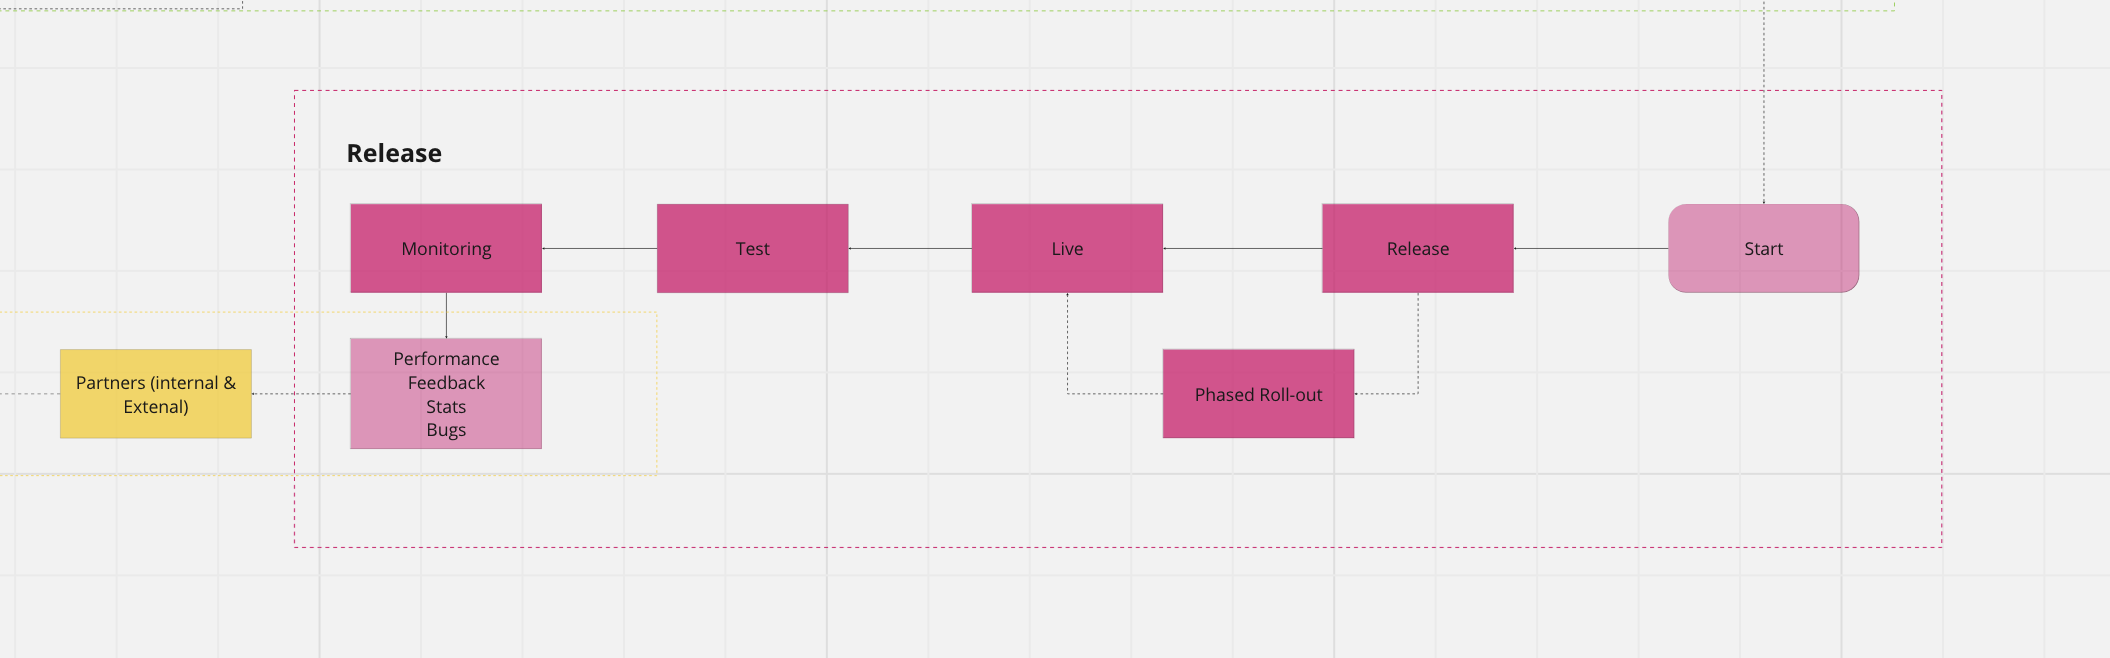
\includegraphics[width=8cm]{assets/workflow/release.png}
    \caption{Release stage of our ways of working.}
    \label{fig:workflowRelease}
  \end{figure}

  However in this case it doesn't become available to partners until we have confidence in the new system. We have config for each partner that 
  specifies what data they have access to. In the case of schedules, this includes keyspace information on where the data is retrieved from. As 
  previously discussed in the \hyperref[sec:cicd]{\textbf{Research}} section, the new and old system will run in parallel until our comparison tests 
  convince us that the new system outputs the same as the old {\textbf{SE-K03} - Shows how we managed risks and avoided a big-bang release.}.

  \begin{figure}[H]
    \centering
    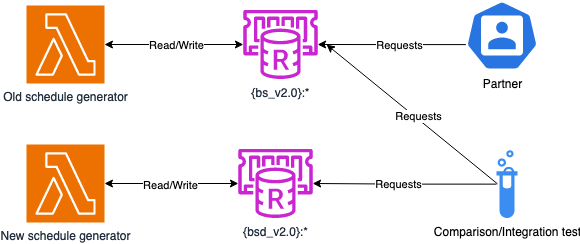
\includegraphics[width=8cm]{assets/keyspaceAccess.drawio.png}
    \caption{Diagram showing access to keyspaces.}
    \label{fig:keySpaceAccess}
  \end{figure}

  Until then partners will still access data from the old system, with a simple config change being the rollover/rollback mechanism. If we wanted we 
  could setup an automatic rollback and huddle system (Sathre, Zambreno, 2008), with the huddle portion consisting of developers being called out if 
  outside of working hours to monitor and remedy the situation. This can be done in many ways but one way would be through AWS alarm 
  actions (Amazon Web Services, 2024i). An alarm going into error would  triggers a rollback of the configs version in S3 (Amazon Web Services, 2024d).

  \begin{figure}[H]
    \centering
    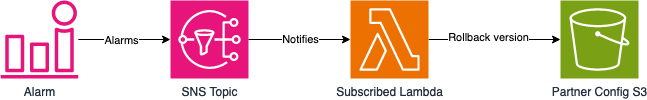
\includegraphics[width=8cm]{assets/rollback.drawio.png}
    \caption{Automatic rollback architecture on alarm error.}
    \label{fig:rollback}
  \end{figure}

  For our case this is most likely over-engineering and unnecessary. A config change only takes a minute to do and if there ever was an error we 
  would be notified and called out to fix the problem when necessary. 

  Once the switchover happens we wait for partner feedback and use created dashboards, these will be shown in the next section, to monitor 
  the new software. Alongside this, our comparison test and side-by-side running of new and old systems will continue for a short while after release, 
  allowing an easy rollback to the old system. Next this old lambdas scheduler will be disabled, but the lambda itself kept in case of an emergency. 
  Finally, after sufficient time has passed the old system can be deconstructed and removed completely.

\newpage


  \newpage
  
  